\chapter{Implementación (I): Metodología y Tecnologías de Soporte}
\label{cap5a}
%\addcontentsline{toc}{chapter}{Implementación (I): Metodología y Tecnologías de
%Soporte}

\begin{flushright}
\begin{minipage}{7.85cm}
    {\em La ingeniería de software se presenta a sí misma como otra causa
    valiosa, pero es un colirio.} \\ Edsger W. Dijkstra
\end{minipage}
\end{flushright}

\vspace*{5mm}

\section{Introducción}

Al ser este un proyecto de tamaño considerable, y al realizarse en grupo, es
necesario establecer una metodología para evitar el trabajo inútil o redundante.

Para organizar nuestro trabajo, y poder mantener siempre cierto control sobre la
evolución de la aplicación, nos hemos servido tanto de herramientas como de
algunas buenas prácticas.

Habiendo desarrollado nuestro proyecto en el marco del IV CUSL\footnote{Concurso
Universitario de Software Libre: \url{http://www.concursosoftwarelibre.org}}
hemos seguido una política de divulgación de la información y unos plazos de
entrega. Desde la organización del concurso pusieron a nuestra disposición una
forja, en concreto la forja
IRIS-Libre\footnote{\url{https://forja.rediris.es/projects/cusl4-catastrof/}},
gracias a la que pudimos agilizar y centralizar las labores de administración y
planificación del proyecto.

Además adoptamos una política de entrevistas frecuentes con los tutores para
así motivarnos y que nos aconsejaran sobre el mejor paso a seguir, o en dónde
deberíamos profundizar más, o cuándo seguir otras vías de investigación.

De esta manera teníamos objetivos a corto plazo, herramientas para la
planificación gracias al IV CUSL, y guía por parte de los tutores.

\section{Metodologías Ágiles}

Una buena planificación no implica el éxito, pero por lo menos te asegura unos
resultados mínimos.

No hemos aplicado ninguna metodología en concreto, si no un conjunto de técnicas
y buenos métodos. Creemos en una metodología de desarrollo ágil.

\subsection{Reuniones de Desarrollo}

Lo principal es la comunicación entre los desarrolladores, para ello decidimos
reunirnos y comentar las avances o principales problemas al menos dos veces a
la semana.

Las reuniones no tenían por qué ser en persona, ni muy formales, podían
realizarse a través de mensajería instantánea, ayudados con herramientas de
pizarras virtuales. De esta forma siempre se tiene una idea muy cercana del
desarrollo del proyecto sin perder mucho tiempo.

Además mantiene un fuerte lazo entre los desarrolladores y les permite ayudarse
unos a otros, evitando así estancamientos o frustraciones con problemas
difíciles.

\subsection{Reuniones con los Tutores}

Nos reuníamos con nuestros tutores al menos dos veces al mes, dependiendo del
ritmo de trabajo y progresos. Estas reuniones eran de carácter informativo y
orientativo.

Las reuniones permiten un crecimiento guiado y controlado del producto final, y
un nivel de acabado mayor al centrarnos solo en las partes realmente importantes
de la investigación y el desarrollo para los objetivos del proyecto.

\subsection{Sistema Incremental}

Lo principal era desarrollar una plataforma muy básica y sencilla donde se
pudieran llevar a cabo pruebas, y una vez completada, ir aumentando las
prestaciones en forma de módulos o complementos que fueran implementando las
funcionalidades deseadas.

Seguimos pues un modelo iterativo de desarrollo del software, que es el ciclo
de vida del software que probablemente mejor se adapte a metodologías ágiles.

\begin{figure}[H]
 \centering
 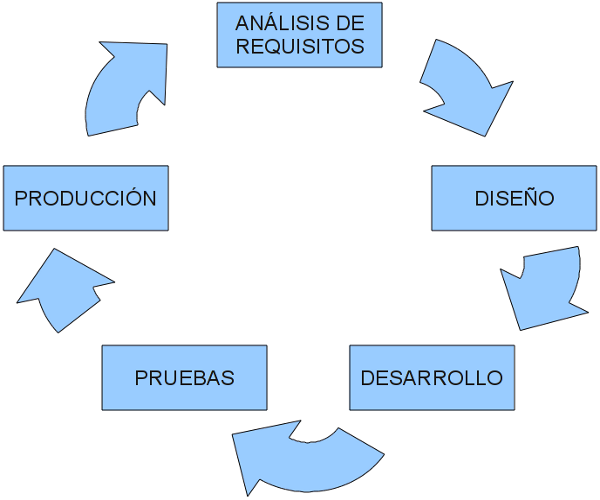
\includegraphics[width=100mm]{figuras/cap5/iterative.png}
 \caption{Ciclo de vida iterativo del software}
\end{figure}

\subsection{Reparto de Tareas Dinámico}

El reparto de tareas equitativo y ágil es vital para mantener una buena
relación entre los desarrolladores, y para el adecuado progreso del proyecto.

Por ello es importante identificar las tareas a realizar e ir asignándolas a
los desarrolladores, de forma que ellos mismos puedan decidir cómo organizarse,
pero siempre teniendo en cuenta unos plazos finales.

El reparto no siempre es estático, puesto que las tareas se pueden alargar o
acortar debido a una mala estimación inicial, incluso a veces se pueden
reasignar o subdividir para agilizar el desarrollo.

Al haber más de un desarrollador en el proyecto hemos tendido un poco a la
especialización en las tareas. Si un desarrollador ha estado trabajando en una
parte, o tiene experiencia y aptitudes para determinado aspecto del desarrollo,
tendrá prioridad a la hora de asignar las tareas relacionadas.

Sin embargo, no se trata de dividir el proyecto en dos, puesto que siempre se
intenta que todos los desarrolladores estén implicados en todas las ramas.
Después de todo el objetivo final del proyecto es aprender y ampliar
conocimientos en todas las áreas que éste toca.

\section{Forja IRIS-Libre}

RedIRIS proporciona un servicio de forja bajo el nombre de
IRIS-Libre\footnote{\url{https://forja.rediris.es/}}. Esta forja proporciona
alojamiento y herramientas a proyectos de Software Libre, y está asociada al
CUSL, dando alojamiento a los proyectos participantes.

\begin{figure}[H]
 \centering
 
\includegraphics[width=30mm]{figuras/cap5/iris_libre.png}
 \caption{Logo de IRIS-Libre}
\end{figure}

Entre las herramientas para el alojamiento y la gestión de proyectos de carácter
colaborativo, y con vistas de crear una comunidad de desarrolladores, que
proporciona encontramos:

\subsection{Subversion}

Como sistema de control de versiones la forja proporciona
SVN\footnote{\url{http://subversion.tigris.org/}}, este sistema permite llevar
un control sobre los cambios en el código, y obtener siempre una copia
actualizada con la última versión.

\begin{figure}[H]
 \centering
 
\includegraphics[width=80mm]{figuras/cap5/svn.png}
 \caption{Logo de Subversion}
\end{figure}

Este tipo de software es imprescindible cuando se trabaja en grupo, pues
facilita la colaboración y permite mantener un orden en el desarrollo.

\subsection{Planificador de Tareas}

La forja también dispone de una sencilla aplicación de control de tareas, que,
entre otras cosas, lo que permite es:

\begin{enumerate}
 \item Crear una tarea, con una breve descripción de la misma.
 \item Asignarlas a un desarrollador, y así poder repartir la carga de trabajo.
 \item Estimación del tiempo necesario, para poder planificar otras tareas.
 \item Progreso de la tarea, para poder hacer un seguimiento del progreso de la
 misma.
 \item Fecha límite de finalización.
\end{enumerate}

Con estos sencillos parámetros la herramienta incluso genera un diagrama de
Gantt para ayudarte con la planificación.

% TODO incluir dicho diagrama?

\section{Blog}

La decisión de comenzar un blog para registrar la evolución del proyecto viene
motivada por el CUSL, que lo exige como requisito de los proyectos
participantes.

El llevar al día un blog\footnote{Simulación de Catástrofes:
\url{http://pfc.mensab.com/}}, con las actualizaciones y las direcciones
generales de desarrollo del proyecto, es algo altamente recomendable si se
quiere que el proyecto cree una comunidad. Es una manera muy cómoda y eficaz de
mantener a la comunidad informada de los cambios y el estado del proyecto.

Además también tiene otras consecuencias más sutiles; por ejemplo, permite
reafirmar las decisiones de diseño o de desarrollo tomadas a lo largo de la
implementación, puesto que queda constancia de las decisiones tomadas y las
razones para llevarlas a cabo.

\section{Git}

Git\footnote{Git - Fast Version Control System: \url{http://git-scm.com/}} es
un sistema de control de versiones distribuido con filosofía distinta a la de
SVN, que es centralizado.

\begin{figure}[H]
 \centering
 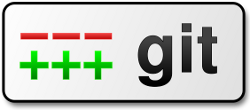
\includegraphics[width=40mm]{figuras/cap5/git.png}
 \caption{Logo de Git}
\end{figure}

En cada proyecto colaborativo hay muchos desarrolladores que necesitan hacer
muchos cambios, probar muchas alternativas de su código y sin embargo mantener
a todo el mundo informado y a su vez mantener una rama estable de desarrollo.
SVN no es demasiado eficiente a la hora de gestionar diferentes ramas de
desarrollo, ni al crearlas ni al unirlas.

Git soluciona este problema al fomentar los {\em commits} pequeños y una
herramienta de {\em merge} más eficiente, lo que facilita trabajar con ramas y
mantenerlas muy fácilmente. El trabajo con diferentes ramas de desarrollo y
una rama {\em master} siempre funcional, de fácil integración entre sí, facilita
el desarrollo considerablemente. Git fomenta este estilo de desarrollo.

Con su sistema de log y sus normas de estilo mejora el seguimiento de todos los
cambios, muy bien documentados, del código.

Por estas razones decidimos migrar la aplicación de SVN a Git cuando terminó el
CUSL. Esta migración nos obligó a buscar una nueva forja que nos proporcionara
este avanzado sistema de control de versiones. La elegida fue
Gitorious\footnote{\url{http://gitorious.org/}}, forja libre para proyectos
libres.

\begin{figure}[H]
 \centering
 
\includegraphics[width=40mm]{figuras/cap5/gitorious.png}
 \caption{Logo de Gitorious}
\end{figure}

%%% Local Variables:
%%% mode: latex
%%% TeX-master: "../dissim"
%%% End: